\chapter{Metamorphic Malware}

The main goal of metamorphism is to change the appearance of the virus while keeping its functionality. These viruses transform their code as they propagate in the system. These viruses evade the risk of signature based detection. Metamorphic viruses use various metamorphic techniques like code permutation, garbage code insertion, etc. 

Metamorphic virus as described in [6], does not have a decryptor and neither a constant body like polymorphic virus. However, they are able to create new generation that look different. Metamorphic viruses usually create new generations that look different from their parents.

The units for model of anatomy of metamorphic engine published in [7] are as follows:

\begin{figure}[htb]
\centering
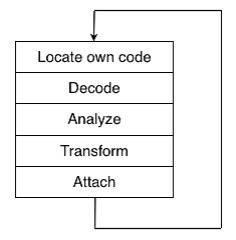
\includegraphics[width=0.4\textwidth]{images/metamorphic_engine.jpg}
\caption{Units in metamorphic model} 
\label{fig: Units in metamorphic model}
\end{figure}

\textbf{Locate own code:} It is important that the metamorphic viruses are able to locate their own code in each new generation. 
 
\textbf{Decode:} The engine needs to decode the information that is required to perform the transformations. The engine must have some depiction of itself in order to know how to make transformations to itself. It may be required to decode other types of information, needed for analysis or transformation. This information can be encoded in the code itself, in data segments or in the virus body.

\textbf{Analyze:} In order to perform metamorphic transformations correctly, some information must be accessible. The register liveliness information is needed for performance of some transformations. If it is not available, the engine must be able to construct such information by itself.

\textbf{Transform:} Metamorphic code transformation without changing the functionality occurs at this point. Instructions blocks are replaced with equivalent blocks at this stage.

\textbf{Attach:} The last step is to attach a new generation of the virus to a new host file. The execution of the units of the metamorphic engine might not be in the order as in the figure. They can be randomly executed. 

The book of "Art of Computer Virus Research and Defense" [1] denotes metamorphic malware as:
\break
\begin{figure}[htb]
\centering
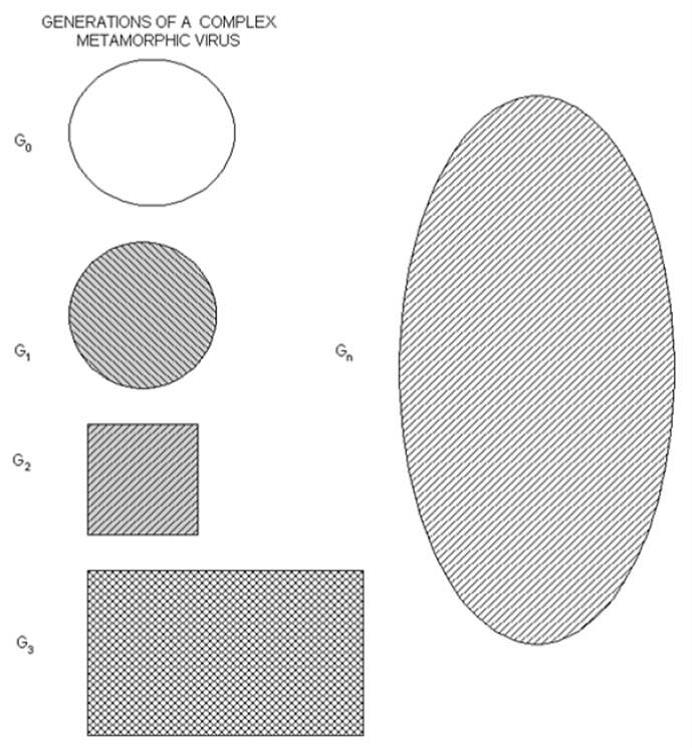
\includegraphics[width=0.8\textwidth]{images/metamorphic_malware.jpg}
\caption{Metamorphic malware} 
\label{fig:Metamorphic malware}
\end{figure}

In the figure above, each subsequent generations of the virus G $(G_1, G_2, G_3....G_n)$ will change their byte patterns to appear different from each other but will functionally be the same. This will evade the signature based detection of the virus. 
\pagebreak
\section{Techniques for generation of metamorphic malware}
The techniques used to create metamorphic virus are as follows:

\subsection{Garbage code insertion}
Garbage code insertion is a simple technique used by many metamorphic and polymorphic viruses to evolve the code. The idea behind this technique is to make their code look different so that no usable hexadecimal search string can be extracted [3]. The functionality of the code is not affected by garbage code insertion.

The Win95/Evol virus used dead code insertion. The two versions of the virus look completely different, but their functions are same. Both transfer two double words into the memory address specified by esi. It is not possible to find common sequence of bytes in both to use as a signature string of the virus. The following code taken from [3] shows dead code insertion used in Win95/Evol virus:

\begin{verbatim}
a. An early generation:

C7060F000055       mov     dword ptr [esi],5500000Fh
C746048BEC5151     mov     dword ptr [esi+0004],5151EC8Bh

b. And one of its later generations:

BF0F000055         mov     edi,5500000Fh
893E               mov     [esi],edi
5F                 pop     edi
52                 push    edx
B640               mov     dh,40
BA8BEC5151         mov     edx,5151EC8Bh
53                 push    ebx
8BDA               mov     ebx,edx
895E04             mov     [esi+0004],ebx
\end{verbatim}

A more advanced from of garbage code insertion is performed by the Win95/Bistro virus, which appeared in October 2000 [1]. In this virus, upon activation of random routine, a "do-nothing" code block is created at the entry-point of the virus.   

\subsection{Register swap}
Register usage exchange is another simple technique used by metamorphic viruses. Different generations of the virus will use the same code, but with different registers. This method was used by the Win95/Reswap virus. The two different generations of Win95/Regswap virus as published in [3] are as follows:

\begin{verbatim}
a.)
5A                       pop   edx
BF04000000               mov   edi,0004h
8BF5                     mov   esi,ebp
B80C000000               mov   eax,000Ch
81C288000000             add   edx,0088h
8B1A                     mov   ebx,[edx]
899C8618110000           mov   [esi+eax*4+00001118],ebx

b.)
58                       pop   eax
BB04000000               mov   ebx,0004h
8BD5                     mov   edx,ebp
BF0C000000               mov   edi,000Ch
81C088000000             add   eax,0088h
8B30                     mov   esi,[eax]
89B4BA18110000           mov   [edx+edi*4+00001118],esi
\end{verbatim}

It can be seen that \lq move edi, 004h\rq\: is replaced by the \lq move ebx, 004h\rq. Similarly, \lq move eax, 000Ch\rq\: is replaced by \lq move edi, 000Ch\rq.

\subsection{Subroutine Permutation}
In this metamorphic technique, the virus code is constant. The code is divided into frames, and then the frames are positioned randomly and connected by branch instructions to preserve the process flow. The branch instructions can be simple or complex, but the flow of control always remains the same.

TheWin32/Ghost and the Win95/Zperm were among the first viruses that used permutation techniques. The Win32/Ghost virus, re-ordered its own subroutines from generation to generation. If there are n subroutines, the different number of possible generations of the virus are n!. The Win32/Ghost had 10 subroutines, thus the total number of virus generations possible are 3628800. Another example of virus that uses subroutine permutation is BadBoy. It has 8 subroutines and hence the total number of generations possible are 40320. The BadBoy virus uses subroutine permutation. The subroutines on the left are the original subroutines whereas those on the right are the permuted ones. The figure below taken from [6] shows its subroutines:

\begin{figure}[htb]
\centering
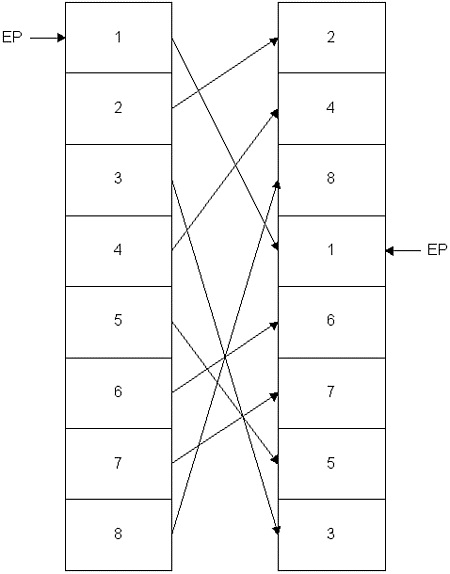
\includegraphics[width=0.6\textwidth]{images/badboy.jpg}
\caption{Badboy subroutines} 
\label{fig: Badboy subrotines}
\end{figure}

\subsection{Random jump instructions}
Another technique to generate metamorphic code is to introduce jumps at random places in the code. The sequence of the execution of the virus always remains the same irrespective of the randomness of the jumps. The Win95/Zperm virus is a good example. The virus inserts and removes jump instructions within its code. Each jump instruction will point to a new instruction of the virus. Zperm never generates a constant body, to avoid the detection of the virus using search string. For this, it also does not generate virus body even in memory. The following figure taken from [6] shows the ZPerm jump instruction insertion:  

\begin{figure}[htb]
\centering
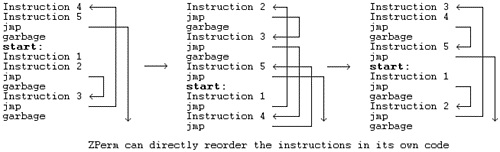
\includegraphics[width=1.0\textwidth]{images/zperm.jpg}
\caption{Zperm random jump instructions} 
\label{fig:Zperm random jump instructions}
\end{figure}

\subsection{Equivalent code substitution}
Some viruses are capable of replacing some instructions with other equivalent instructions. Win95/Zperm has the ability to perform instruction replacement. For example, "sub eax, eax" which also zeroes the contents of the eax register, will replace the instruction, "xor eax, eax". Both these instructions are functionally the same, but have different opcodes. 

Another example of a virus that uses instruction replacement is Win95/Zmist. The types of replacements performed by Zmist, as described in [8] are:
\begin{itemize}
\item reversing of branch conditions
\item register moves replaced by push/pop sequences 
\item alternative opcode encoding 
\item xor/sub and or/test interchanging
\end{itemize}

Win95/Bistro performs similar replacements. Here is the original code of a target before processing by Bistro as in [6]: 
\begin{verbatim}
Before:
55          push    ebp
8BEC        mov     ebp, esp
8B7608      mov     esi, dword ptr [ebp + 08]
85F6        test    esi, esi
743B        je      401045
8B7E0C      mov     edi, dword ptr [ebp + 0c]
09FF        or      edi, edi
7434        je      401045
31D2        xor     edx, edx

After :
55          push    ebp
54          push    esp			            register move replaced by push/pop
5D          pop     ebp			            register move replaced by push/pop
8B7608      mov     esi, dword ptr [ebp + 08] 
09F6        or      esi, esi			    test/or interchange
743B        je      401045
8B7E0C      mov     edi, dword ptr [ebp + 0c]
85FF        test    edi, edi			    test/or interchange
7434        je      401045
28D2        sub     edx, edx	            xor/sub interchange
\end{verbatim}

\subsection{Host code mutation}
The Win95/Bistro virus not only mutates itself in new generations, but it also mutates the code of its host. The virus is thus able to generate new viruses and worms. The virus uses a randomly executed code morphing routine in order to do this. The instance of Bistro is described in the previous section. Also, because the entry-point code of the application could be different, disinfection cannot be done perfectly. 
